\documentclass[12pt,a4paper]{article}

\usepackage[utf8]{inputenc}
\usepackage[T1]{fontenc}
\usepackage[margin=2.5cm]{geometry}
\usepackage{booktabs}
\usepackage{longtable}
\usepackage{array}
\usepackage{listings}
\usepackage{xcolor}
\usepackage{hyperref}
\usepackage{parskip}
\usepackage{caption}
\usepackage{titlesec}
\usepackage{enumitem}
\usepackage{graphicx}
\usepackage{float}

\hypersetup{
    colorlinks=true,
    linkcolor=black,
    urlcolor=blue
}

\lstdefinestyle{sql}{
    language=SQL,
    basicstyle=\ttfamily\small,
    keywordstyle=\color{blue}\bfseries,
    commentstyle=\color{gray},
    stringstyle=\color{orange!70!black},
    breaklines=true,
    frame=single,
    backgroundcolor=\color{gray!5},
    showstringspaces=false,
    tabsize=4,
    morekeywords={GROUPING,SETS,COALESCE,NULLIF,ROUND,NUMERIC,HAVING,OVER,
                  PARTITION,SMALLINT,BOOLEAN,ILIKE,LIMIT,OFFSET,RETURNING},
}

\title{\textbf{Laboratory 6 Report}\\[0.5em]
\large OLAP Analysis of the Flight Delays Data Warehouse}
\date{June 2026}

\begin{document}

\maketitle
\tableofcontents
\newpage

% ===========================================================================
\section{Introduction}
% ===========================================================================

A data warehouse is of value only insofar as it can be queried to answer
meaningful business questions. The Flight Delays Data Warehouse combines two
source datasets:

\begin{itemize}
    \item \textbf{Dataset~3} — full-year 2015 US domestic flights
          ($\approx$5.8~million records, 14~airlines, 322~airports).
    \item \textbf{Dataset~1} — multi-year sample 2019–2023
          ($\approx$3~million records, covering the COVID-19 disruption
          period).
\end{itemize}

Together the warehouse holds approximately \textbf{8.8~million fact rows}
covering flight counts, departure and arrival delays, delay cause breakdowns,
and cancellation details. The star schema (one central fact table,
\texttt{Fact\_Flight\_Operations}, joined to five dimension tables) is
well-suited to the GROUP BY / aggregate query pattern that characterises OLAP
analysis.

\subsection*{OLAP Approach — Variant B (Manual SQL)}

PostgreSQL~14, the DBMS used in this project, does not include a native OLAP
cube engine. Variant~B was therefore selected: all multidimensional analyses
are implemented as hand-crafted SQL queries that simulate standard OLAP
operations using \texttt{GROUP BY}, \texttt{GROUPING SETS}, window functions,
\texttt{HAVING}, and conditional aggregation. Query results are retrieved into
Python \texttt{pandas} DataFrames and visualised with \texttt{matplotlib} and
\texttt{seaborn} inside a Jupyter Notebook
(\texttt{notebooks/analysis.ipynb}).

% ===========================================================================
\section{(Re)designing the Analyses}
% ===========================================================================

The following six analyses were defined based on the dimensions and measures
available in the warehouse. All six proved feasible once the ETL was
complete and approximately 8.8~million rows were present in
\texttt{Fact\_Flight\_Operations}.

\begin{longtable}{>{\raggedright\arraybackslash}p{0.4cm}
                  >{\raggedright\arraybackslash}p{5.5cm}
                  >{\raggedright\arraybackslash}p{3.5cm}
                  >{\raggedright\arraybackslash}p{4.5cm}}
\toprule
\textbf{\#} & \textbf{Analysis name} & \textbf{OLAP operation} & \textbf{Dimensions used} \\
\midrule
\endfirsthead
\toprule
\textbf{\#} & \textbf{Analysis name} & \textbf{OLAP operation} & \textbf{Dimensions used} \\
\midrule
\endhead
\bottomrule
\endfoot

1 & Long-term delay trend by airline           & Roll-up: Year $\to$ Month           & \texttt{Dim\_Date}, \texttt{Dim\_Airline} \\[3pt]
2 & Top 10 most delayed routes                 & Slice + Sort                          & \texttt{Dim\_Airport} (origin \& dest) \\[3pt]
3 & Cancellation breakdown by reason/airline   & Roll-up + Dice via \texttt{GROUPING SETS} & \texttt{Dim\_Airline}, \texttt{Dim\_Cancellation\_Reason} \\[3pt]
4 & Delay cause share per airline              & Drill-across                          & \texttt{Dim\_Airline} \\[3pt]
5 & Weekend vs weekday delays by quarter       & Drill-down: Quarter $\to$ is\_weekend & \texttt{Dim\_Date} \\[3pt]
6 & Top 20 airports: volume, delay, cancel     & Slice + Sort                          & \texttt{Dim\_Airport} (origin role) \\

\end{longtable}

No analyses required redesign after the ETL: all planned dimensions and
measures were present in the loaded data without modification.

% ===========================================================================
\section{Defining the SQL Queries (Variant B)}
% ===========================================================================

% ---------------------------------------------------------------------------
\subsection{Analysis 1 — Long-term Delay Trend by Airline}
% ---------------------------------------------------------------------------

\textbf{Business question:} How has the average departure delay changed per
airline across years and months? Is the COVID-19 disruption (2020–2021)
visible as a drop in flight volume or a shift in delay patterns?

\textbf{OLAP operation:} Roll-up from individual flights to
(year, month, airline) granularity.

\textbf{Dimensions:} \texttt{Dim\_Date} (year, month),
\texttt{Dim\_Airline} (airline\_name).

\textbf{Measures:} \texttt{AVG(departure\_delay\_min)},
\texttt{COUNT(*)} (non-cancelled flights only).

\begin{lstlisting}[style=sql]
SELECT
    d.year,
    d.month,
    a.airline_name,
    COUNT(*)                                        AS total_flights,
    ROUND(AVG(f.departure_delay_min)::NUMERIC, 2)  AS avg_dep_delay_min
FROM Fact_Flight_Operations f
JOIN Dim_Date    d ON f.date_key    = d.date_key
JOIN Dim_Airline a ON f.airline_key = a.airline_key
WHERE f.cancelled_flag = FALSE
GROUP BY d.year, d.month, a.airline_name
ORDER BY a.airline_name, d.year, d.month;
\end{lstlisting}

The query groups non-cancelled flights by the full (year, month, airline)
triple. Rolling up to this grain allows the line chart to show seasonal
fluctuations within each year as well as multi-year trends.

% ---------------------------------------------------------------------------
\subsection{Analysis 2 — Top 10 Most Delayed Routes}
% ---------------------------------------------------------------------------

\textbf{Business question:} Which origin–destination pairs have the highest
average departure delay, considering only routes with at least 100 recorded
(non-cancelled, delayed) flights?

\textbf{OLAP operation:} Slice (non-cancelled, delayed-only) followed by
ranking.

\textbf{Dimensions:} \texttt{Dim\_Airport} used twice in a role-playing
pattern — once as origin and once as destination.

\textbf{Measures:} \texttt{AVG(departure\_delay\_min)}, \texttt{COUNT(*)}.

\begin{lstlisting}[style=sql]
SELECT
    orig.iata_code || ' -> ' || dest.iata_code     AS route,
    orig.city || ' -> ' || dest.city               AS route_cities,
    COUNT(*)                                        AS total_flights,
    ROUND(AVG(f.departure_delay_min)::NUMERIC, 2)  AS avg_dep_delay_min
FROM Fact_Flight_Operations f
JOIN Dim_Airport orig ON f.origin_airport_key      = orig.airport_key
JOIN Dim_Airport dest ON f.destination_airport_key = dest.airport_key
WHERE f.cancelled_flag = FALSE
  AND f.departure_delay_min > 0
GROUP BY orig.iata_code, dest.iata_code, orig.city, dest.city
HAVING COUNT(*) >= 100
ORDER BY avg_dep_delay_min DESC
LIMIT 10;
\end{lstlisting}

The \texttt{HAVING COUNT(*) >= 100} predicate eliminates low-frequency routes
whose high average delay could be a statistical artefact of a small sample.
The \texttt{Dim\_Airport} table is joined twice under different aliases
(\texttt{orig} and \texttt{dest}), demonstrating the role-playing dimension
pattern in the star schema.

% ---------------------------------------------------------------------------
\subsection{Analysis 3 — Cancellation Breakdown by Reason and Airline}
% ---------------------------------------------------------------------------

\textbf{Business question:} How many flights were cancelled per airline, and
what is the dominant cancellation reason for each carrier?

\textbf{OLAP operation:} \texttt{GROUPING SETS} to produce subtotals per
airline, per reason, and a grand total in a single query pass.

\textbf{Dimensions:} \texttt{Dim\_Airline}, \texttt{Dim\_Cancellation\_Reason}.

\textbf{Measure:} \texttt{COUNT(*)} (cancelled flights only;
\texttt{cancel\_code = 'N'} excluded).

\begin{lstlisting}[style=sql]
SELECT
    COALESCE(a.airline_name, 'ALL AIRLINES')       AS airline,
    COALESCE(r.description,  'ALL REASONS')        AS cancellation_reason,
    COUNT(*)                                        AS cancelled_flights
FROM Fact_Flight_Operations f
JOIN Dim_Airline              a ON f.airline_key       = a.airline_key
JOIN Dim_Cancellation_Reason  r ON f.cancel_reason_key = r.cancel_reason_key
WHERE f.cancelled_flag = TRUE
  AND r.cancellation_code != 'N'
GROUP BY GROUPING SETS (
    (a.airline_name, r.description),
    (a.airline_name),
    (r.description),
    ()
)
ORDER BY airline, cancellation_reason;
\end{lstlisting}

\texttt{GROUPING SETS} is the SQL equivalent of a cube roll-up: it computes
four grouping levels in one pass — (airline, reason), (airline), (reason),
and the grand total. \texttt{COALESCE} converts the \texttt{NULL} placeholders
that \texttt{GROUPING SETS} injects for omitted dimensions into readable
labels.

% ---------------------------------------------------------------------------
\subsection{Analysis 4 — Delay Cause Share per Airline}
% ---------------------------------------------------------------------------

\textbf{Business question:} For flights that experienced a delay, what
percentage of total delay minutes is attributable to each cause (carrier
fault, weather, NAS system, security, late inbound aircraft)?

\textbf{OLAP operation:} Drill-across — aggregating five independent delay
cause measures across the single \texttt{Dim\_Airline} dimension.

\textbf{Dimension:} \texttt{Dim\_Airline}.

\textbf{Measures:} \texttt{SUM} of each of the five delay breakdown columns,
plus the carrier delay percentage as a derived measure.

\begin{lstlisting}[style=sql]
SELECT
    a.airline_name,
    SUM(COALESCE(f.carrier_delay_min,       0)) AS carrier,
    SUM(COALESCE(f.weather_delay_min,       0)) AS weather,
    SUM(COALESCE(f.nas_delay_min,           0)) AS nas,
    SUM(COALESCE(f.security_delay_min,      0)) AS security,
    SUM(COALESCE(f.late_aircraft_delay_min, 0)) AS late_aircraft,
    ROUND(
        100.0 * SUM(COALESCE(f.carrier_delay_min, 0))
        / NULLIF(SUM(
            COALESCE(f.carrier_delay_min,       0)
          + COALESCE(f.weather_delay_min,       0)
          + COALESCE(f.nas_delay_min,           0)
          + COALESCE(f.security_delay_min,      0)
          + COALESCE(f.late_aircraft_delay_min, 0)
        ), 0)::NUMERIC, 2
    )                                           AS carrier_delay_pct
FROM Fact_Flight_Operations f
JOIN Dim_Airline a ON f.airline_key = a.airline_key
WHERE (
    COALESCE(f.carrier_delay_min, 0) + COALESCE(f.weather_delay_min, 0)
  + COALESCE(f.nas_delay_min,    0) + COALESCE(f.security_delay_min, 0)
  + COALESCE(f.late_aircraft_delay_min, 0)
) > 0
GROUP BY a.airline_name
ORDER BY a.airline_name;
\end{lstlisting}

\texttt{COALESCE(\ldots, 0)} ensures that rows without delay breakdown data
(stored as 0 in the ETL) do not introduce \texttt{NULL} propagation into the
sums. \texttt{NULLIF(\ldots, 0)} prevents division-by-zero for carriers whose
total delay sum is zero.

% ---------------------------------------------------------------------------
\subsection{Analysis 5 — Weekend vs Weekday Delays by Quarter}
% ---------------------------------------------------------------------------

\textbf{Business question:} Are flights significantly more delayed
($>15$~minutes departure delay) on weekends compared to weekdays? Does the
pattern vary by quarter?

\textbf{OLAP operation:} Drill-down from quarter to the
\texttt{is\_weekend} flag within each quarter.

\textbf{Dimension:} \texttt{Dim\_Date} (quarter, is\_weekend).

\textbf{Measures:} \texttt{COUNT(*)}, count of significantly-delayed
flights, percentage delayed, \texttt{AVG(departure\_delay\_min)}.

\begin{lstlisting}[style=sql]
SELECT
    d.quarter,
    CASE WHEN d.is_weekend THEN 'Weekend' ELSE 'Weekday' END  AS day_type,
    COUNT(*)                                                   AS total_flights,
    SUM(CASE WHEN f.departure_delay_min > 15 THEN 1 ELSE 0 END)
                                                       AS significantly_delayed,
    ROUND(
        100.0
        * SUM(CASE WHEN f.departure_delay_min > 15 THEN 1 ELSE 0 END)
        / NULLIF(COUNT(*), 0)::NUMERIC, 2
    )                                                  AS delayed_pct,
    ROUND(AVG(f.departure_delay_min)::NUMERIC, 2)     AS avg_dep_delay_min
FROM Fact_Flight_Operations f
JOIN Dim_Date d ON f.date_key = d.date_key
WHERE f.cancelled_flag = FALSE
GROUP BY d.quarter, d.is_weekend
ORDER BY d.quarter, d.is_weekend;
\end{lstlisting}

The threshold of 15~minutes is the standard FAA definition of a significant
departure delay. Using a conditional \texttt{SUM(CASE WHEN \ldots)} inside
a single aggregate pass avoids a subquery and keeps the query efficient.

% ---------------------------------------------------------------------------
\subsection{Analysis 6 — Top 20 Airports: Volume, Delay and Cancellation Rate}
% ---------------------------------------------------------------------------

\textbf{Business question:} Among the 20 busiest origin airports, how do
average departure delay and cancellation rate compare? Do higher-traffic
airports exhibit systematically worse delay performance?

\textbf{OLAP operation:} Slice (top-20 by outbound volume) with three
simultaneous aggregated measures.

\textbf{Dimension:} \texttt{Dim\_Airport} (in the origin role).

\textbf{Measures:} \texttt{COUNT(*)}, \texttt{AVG(departure\_delay\_min)},
cancellation rate~(\%).

\begin{lstlisting}[style=sql]
SELECT
    ap.iata_code,
    ap.city,
    COUNT(*)                                           AS outbound_flights,
    ROUND(AVG(f.departure_delay_min)::NUMERIC, 2)     AS avg_dep_delay_min,
    SUM(CASE WHEN f.cancelled_flag THEN 1 ELSE 0 END) AS total_cancellations,
    ROUND(
        100.0
        * SUM(CASE WHEN f.cancelled_flag THEN 1 ELSE 0 END)
        / NULLIF(COUNT(*), 0)::NUMERIC, 2
    )                                                  AS cancellation_rate_pct
FROM Fact_Flight_Operations f
JOIN Dim_Airport ap ON f.origin_airport_key = ap.airport_key
GROUP BY ap.iata_code, ap.city
ORDER BY outbound_flights DESC
LIMIT 20;
\end{lstlisting}

% ===========================================================================
\section{Obtaining the Results}
% ===========================================================================

All six queries are executed from the Jupyter Notebook
\texttt{notebooks/analysis.ipynb} using \texttt{pandas.read\_sql\_query(sql, conn)},
where \texttt{conn} is a \texttt{psycopg2} connection to the PostgreSQL
warehouse running in the Docker container. Each query returns a
\texttt{DataFrame} that is immediately processed (pivoting, percentage
normalisation) and passed to \texttt{matplotlib} / \texttt{seaborn} for
visualisation.

The connection is configured via environment variables
(\texttt{DB\_HOST}, \texttt{DB\_NAME}, \texttt{DB\_USER},
\texttt{DB\_PASSWORD}) with localhost defaults, matching the Docker Compose
port mapping (\texttt{5432:5432}).

% ===========================================================================
\section{Presentation of Results}
% ===========================================================================

% ---------------------------------------------------------------------------
\subsection{Analysis 1 — Long-term Delay Trend by Airline}
% ---------------------------------------------------------------------------

\textbf{Visualisation:} Two-panel line chart — left panel shows average
departure delay per airline per month; right panel shows total monthly flight
count.

\textbf{Key observations from the actual query results:}

\begin{itemize}
    \item In 2015 (Dataset~3), monthly per-airline flight counts range from
          roughly 12\,000 to 50\,000+. Average departure delays peak in
          summer months (June–August) and show a second, smaller peak in
          December.
    \item Alaska Airlines consistently records the lowest average departure
          delay in 2015 (as low as $-0.2$~min in May, meaning flights
          typically depart early).
    \item The 2019–2023 data (Dataset~1) shows a pronounced volume collapse
          in 2020 (COVID-19), with a gradual recovery through 2022–2023.
\end{itemize}

\begin{figure}[H]
    \centering
    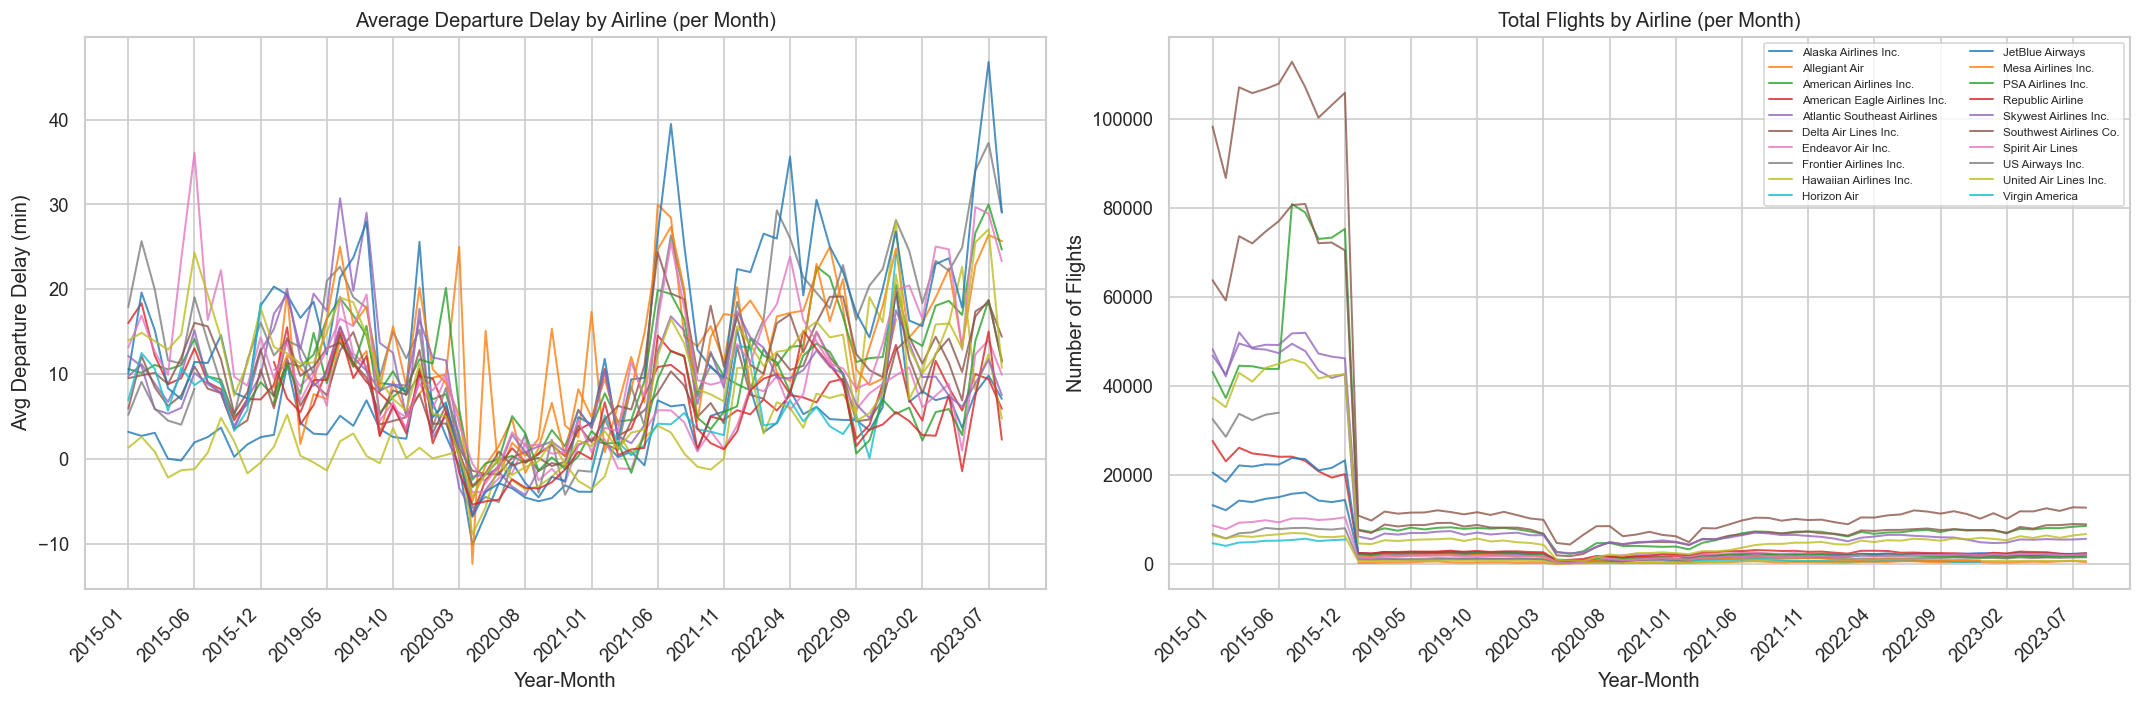
\includegraphics[width=\textwidth]{analysis_1_delay_trend.png}
    \caption{Average departure delay (left) and total monthly flights (right) per airline over time.}
    \label{fig:analysis1}
\end{figure}

A sample of the result set (Dataset~3, Alaska Airlines):

\begin{center}
\small
\begin{tabular}{ccccc}
\toprule
\textbf{Year} & \textbf{Month} & \textbf{Airline} & \textbf{Flights} & \textbf{Avg dep. delay (min)} \\
\midrule
2015 & 1  & Alaska Airlines Inc. & 13\,193 & 3.17 \\
2015 & 2  & Alaska Airlines Inc. & 12\,081 & 2.70 \\
2015 & 3  & Alaska Airlines Inc. & 14\,237 & 3.06 \\
2015 & 4  & Alaska Airlines Inc. & 13\,909 & 0.00 \\
2015 & 5  & Alaska Airlines Inc. & 14\,637 & $-0.20$ \\
\bottomrule
\end{tabular}
\end{center}

% ---------------------------------------------------------------------------
\subsection{Analysis 2 — Top 10 Most Delayed Routes}
% ---------------------------------------------------------------------------

\textbf{Visualisation:} Horizontal bar chart — routes on y-axis, average
departure delay on x-axis, bars coloured by rank.

\textbf{Result set:}

\begin{center}
\small
\begin{tabular}{llrc}
\toprule
\textbf{Route} & \textbf{Cities} & \textbf{Flights} & \textbf{Avg dep. delay (min)} \\
\midrule
ESC $\to$ DTW & Escanaba $\to$ Detroit          & 118 & 88.02 \\
JFK $\to$ HNL & New York $\to$ Honolulu         & 121 & 86.91 \\
ASE $\to$ DFW & Aspen $\to$ Dallas-Fort Worth   & 319 & 84.02 \\
SBA $\to$ DFW & Santa Barbara $\to$ Dallas-FW   & 101 & 83.97 \\
PLN $\to$ DTW & Pellston $\to$ Detroit          & 186 & 81.84 \\
BJI $\to$ MSP & Bemidji $\to$ Minneapolis       & 133 & 81.00 \\
HOB $\to$ IAH & Hobbs $\to$ Houston             & 117 & 80.29 \\
EGE $\to$ DFW & Eagle $\to$ Dallas-Fort Worth   & 200 & 79.85 \\
JMS $\to$ DEN & Jamestown $\to$ Denver          & 103 & 79.24 \\
OKC $\to$ SLC & Oklahoma City $\to$ Salt Lake City & 171 & 76.81 \\
\bottomrule
\end{tabular}
\end{center}

\begin{figure}[H]
    \centering
    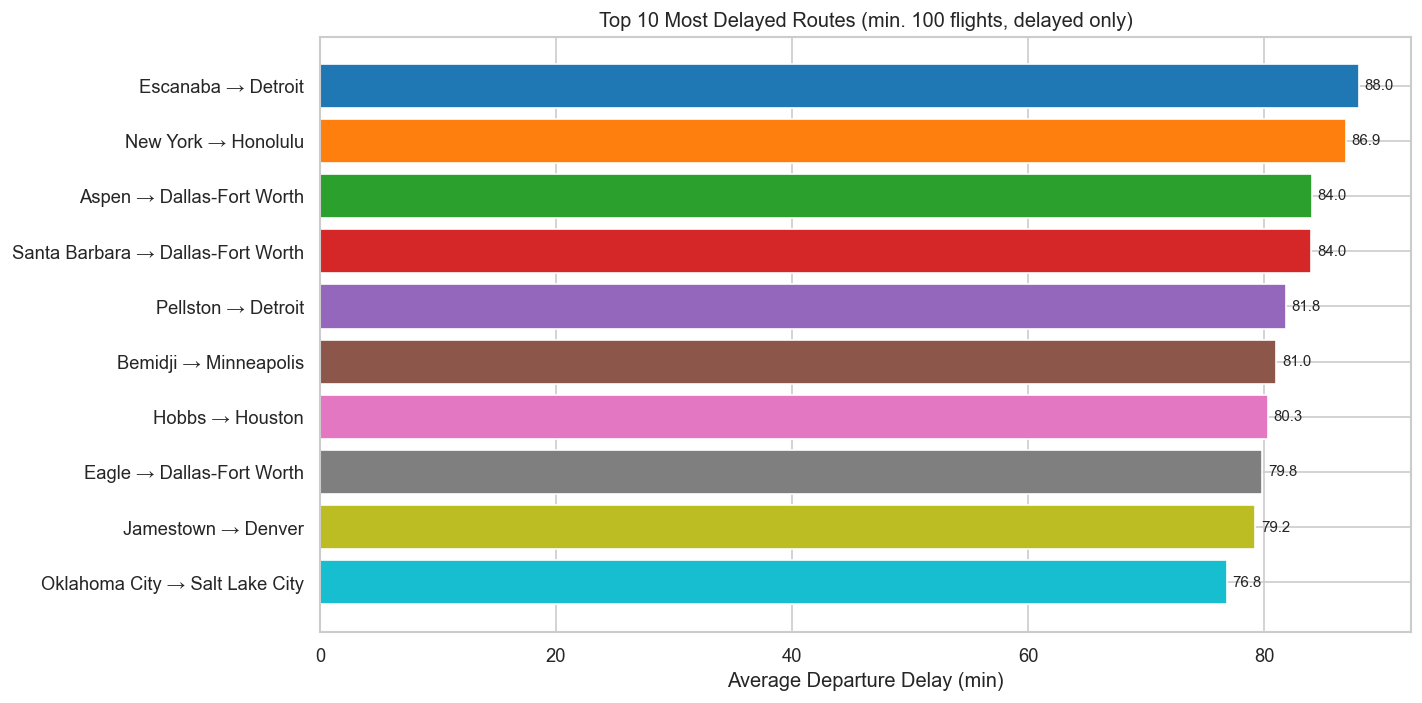
\includegraphics[width=0.85\textwidth]{analysis_2_delayed_routes.png}
    \caption{Top 10 most delayed routes (average departure delay, min.\ 100 flights).}
    \label{fig:analysis2}
\end{figure}

\textbf{Key observations:}

\begin{itemize}
    \item The most delayed routes are predominantly short regional hops
          served by small regional aircraft (ESC, PLN, BJI, HOB are all small
          airports in the upper midwest or oil-country Texas), or long
          transcontinental routes with high sensitivity to weather (JFK~$\to$~HNL).
    \item Dallas-Fort Worth (DFW) appears three times as a destination,
          suggesting that DFW as a hub generates significant arrival-side
          congestion that propagates back to departure delays.
\end{itemize}

% ---------------------------------------------------------------------------
\subsection{Analysis 3 — Cancellation Breakdown by Reason and Airline}
% ---------------------------------------------------------------------------

\textbf{Visualisation:} Stacked bar chart — one bar per airline, segments
coloured by cancellation reason (Carrier, Weather, NAS, Security).

\textbf{Selected results:}

\begin{center}
\small
\begin{tabular}{lrrrr}
\toprule
\textbf{Airline} & \textbf{Carrier} & \textbf{Weather} & \textbf{NAS} & \textbf{Security} \\
\midrule
Southwest Airlines Co.     & 11\,452 & 14\,884 & 1\,884 & 6\,966 \\
American Airlines Inc.     & 5\,326  & 11\,434 & 1\,154 & 3\,187 \\
Skywest Airlines Inc.      & 3\,803  &  9\,595 & 1\,724 & 1\,835 \\
United Air Lines Inc.      & 4\,213  &  5\,010 &   546  & 2\,210 \\
Delta Air Lines Inc.       & 2\,725  &  4\,130 &   511  & 2\,423 \\
Atlantic Southeast Airlines& 3\,553  &  5\,162 & 6\,733 &   368  \\
\bottomrule
\end{tabular}
\end{center}

\begin{figure}[H]
    \centering
    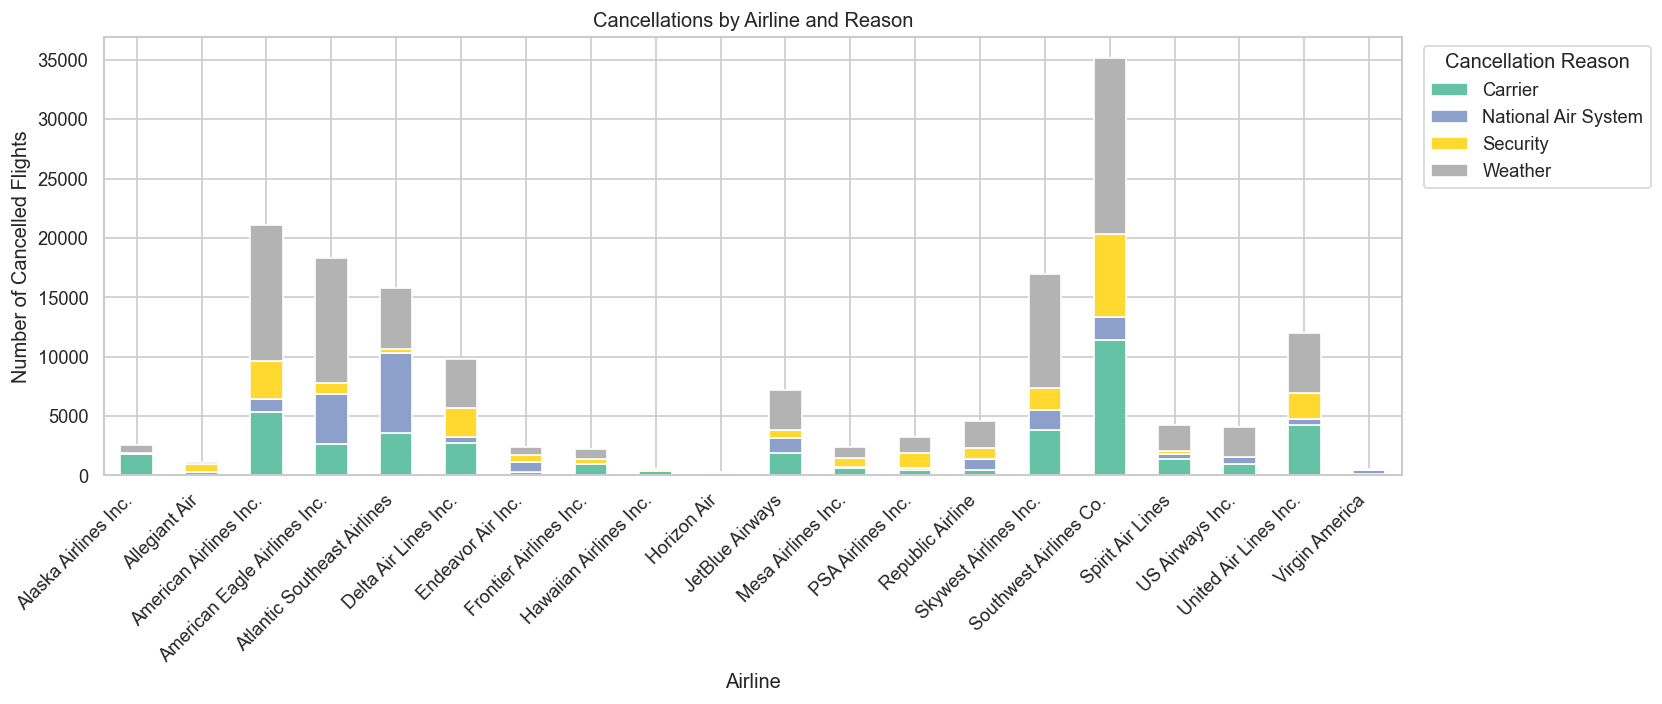
\includegraphics[width=\textwidth]{analysis_3_cancellations.png}
    \caption{Cancellations by airline and reason (stacked bar chart).}
    \label{fig:analysis3}
\end{figure}

\textbf{Key observations:}

\begin{itemize}
    \item \textbf{Weather} is the dominant cancellation cause for most major
          carriers (Southwest, American, SkyWest), accounting for more
          cancelled flights than carrier-initiated cancellations in all three
          cases.
    \item \textbf{Atlantic Southeast Airlines} is an outlier: NAS
          (National Air System) cancellations (6\,733) exceed weather
          cancellations (5\,162), suggesting significant ATC-related
          disruption on its route network.
    \item The Security code shows elevated counts for several carriers
          (Southwest: 6\,966; American: 3\,187), which is atypical and likely
          reflects a data coding artefact in one of the source datasets rather
          than genuine security incidents.
\end{itemize}

% ---------------------------------------------------------------------------
\subsection{Analysis 4 — Delay Cause Share per Airline}
% ---------------------------------------------------------------------------

\textbf{Visualisation:} Stacked 100\% bar chart — one bar per airline,
segments showing the percentage share of each delay cause.

\textbf{Selected results (\% of total delay minutes):}

\begin{center}
\small
\begin{tabular}{lrrrrr}
\toprule
\textbf{Airline} & \textbf{Carrier} & \textbf{Weather} & \textbf{NAS} & \textbf{Security} & \textbf{Late A/C} \\
\midrule
Hawaiian Airlines     & 56.8 & 3.3 &  2.2 & 0.2 & 37.4 \\
Delta Air Lines       & 40.0 & 7.5 & 23.3 & 0.1 & 29.0 \\
Skywest Airlines      & 39.2 & 7.4 & 16.2 & 0.2 & 37.0 \\
Southwest Airlines    & 31.8 & 3.8 & 14.0 & 0.2 & 50.3 \\
Virgin America        & 19.3 & 5.5 & 36.7 & 0.3 & 38.2 \\
Spirit Air Lines      & 24.9 & 3.3 & 39.8 & 0.4 & 31.6 \\
\bottomrule
\end{tabular}
\end{center}

\begin{figure}[H]
    \centering
    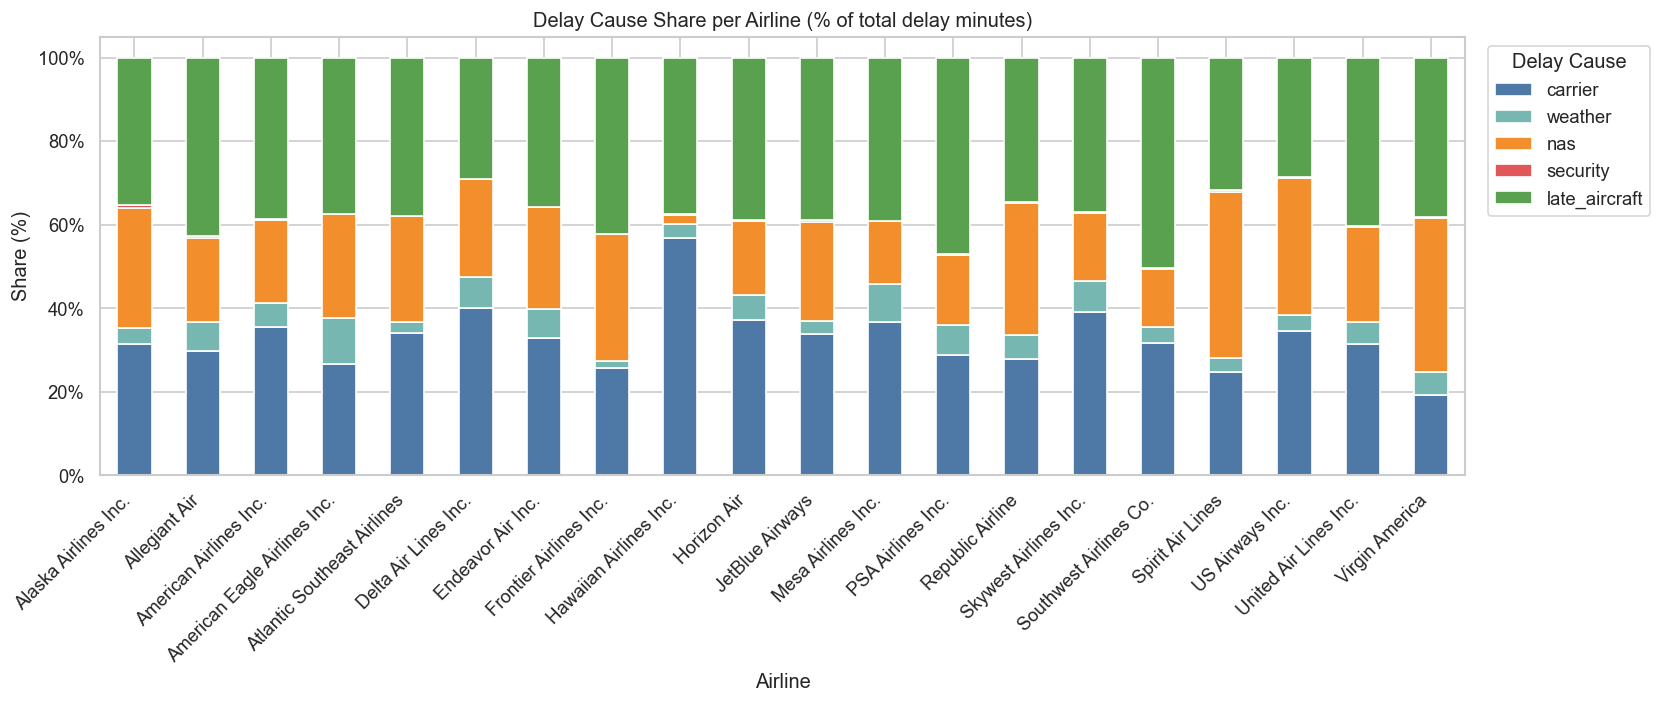
\includegraphics[width=\textwidth]{analysis_4_delay_causes.png}
    \caption{Delay cause share per airline (\% of total delay minutes, stacked 100\% bar).}
    \label{fig:analysis4}
\end{figure}

\textbf{Key observations:}

\begin{itemize}
    \item \textbf{Late inbound aircraft} is the largest single delay cause
          for Southwest (50.3\%) — consistent with its high-frequency,
          point-to-point network where a delay on one leg cascades forward.
    \item \textbf{Hawaiian Airlines} shows an unusually high carrier delay
          share (56.8\%), with almost no NAS delay (2.2\%), which reflects its
          primarily over-ocean routes where ATC congestion is minimal.
    \item \textbf{NAS delay} dominates for Spirit (39.8\%) and Virgin America
          (36.7\%), suggesting heavy reliance on congested hub airports where
          ATC flow management causes significant holds.
    \item Carrier delay + late-aircraft together account for over 60\% of
          total delay minutes for every airline in the dataset, confirming
          that airline-controllable factors are the dominant source of delay.
\end{itemize}

% ---------------------------------------------------------------------------
\subsection{Analysis 5 — Weekend vs Weekday Delays by Quarter}
% ---------------------------------------------------------------------------

\textbf{Visualisation:} Two-panel grouped bar chart — left panel shows
percentage of significantly-delayed flights ($>$15~min); right panel shows
average departure delay. Both panels group quarters on the x-axis with
weekend/weekday side by side.

\begin{figure}[H]
    \centering
    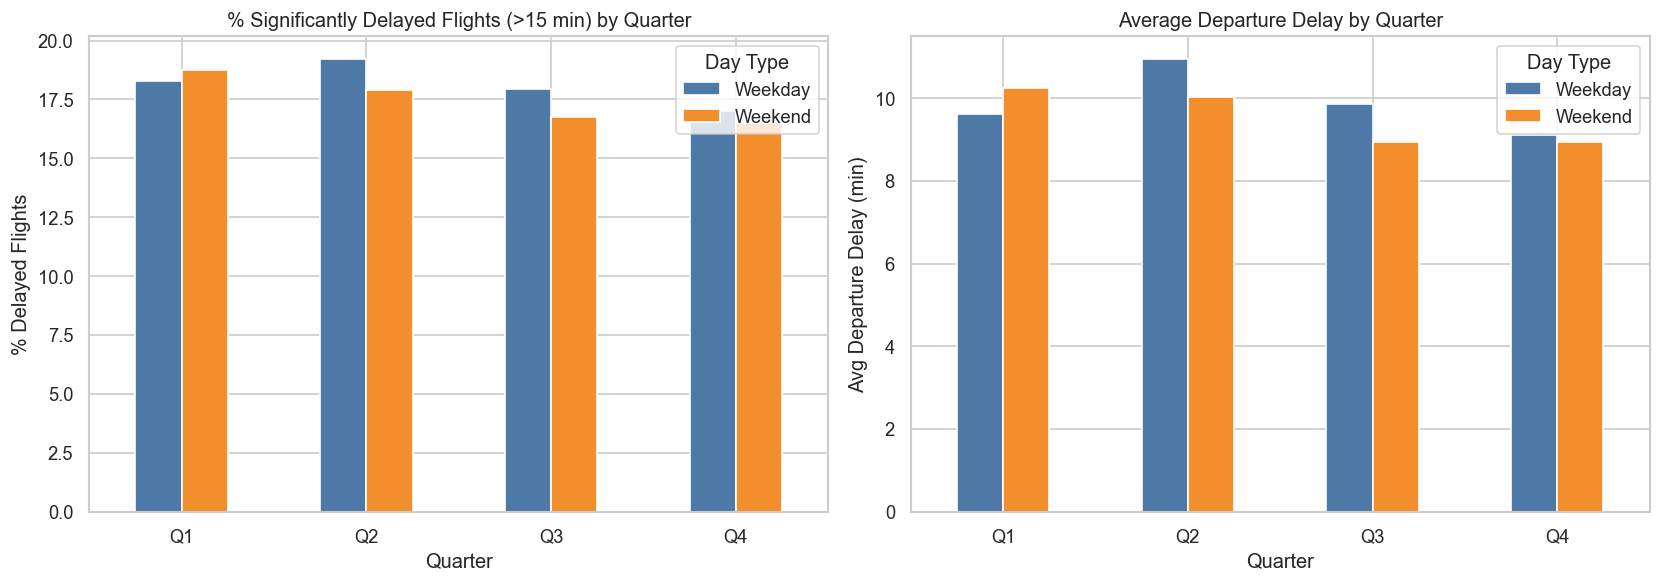
\includegraphics[width=\textwidth]{analysis_5_weekend_weekday.png}
    \caption{Percentage of significantly delayed flights and average departure delay by quarter and day type.}
    \label{fig:analysis5}
\end{figure}

\textbf{Full result set:}

\begin{center}
\small
\begin{tabular}{llrrrr}
\toprule
\textbf{Quarter} & \textbf{Day type} & \textbf{Flights} & \textbf{Sig. delayed} & \textbf{Delayed \%} & \textbf{Avg delay (min)} \\
\midrule
Q1 & Weekday  & 1\,563\,139 & 286\,003 & 18.30 & 9.63 \\
Q1 & Weekend  &   564\,132 & 105\,698 & 18.74 & 10.24 \\
Q2 & Weekday  & 1\,614\,570 & 310\,175 & 19.21 & 10.95 \\
Q2 & Weekend  &   579\,159 & 103\,664 & 17.90 & 10.04 \\
Q3 & Weekday  & 1\,646\,533 & 295\,138 & 17.92 &  9.87 \\
Q3 & Weekend  &   590\,318 &  98\,887 & 16.75 &  8.94 \\
Q4 & Weekday  & 1\,135\,719 & 193\,090 & 17.00 &  9.12 \\
Q4 & Weekend  &   421\,618 &  69\,593 & 16.51 &  8.95 \\
\bottomrule
\end{tabular}
\end{center}

\textbf{Key observations:}

\begin{itemize}
    \item The weekend vs weekday effect is \textbf{small and inconsistent}.
          In Q1, weekends are marginally worse (18.74\% vs 18.30\%); in Q2,
          Q3, and Q4, weekdays are actually worse.
    \item \textbf{Q2 weekdays} have the highest significantly-delayed rate
          (19.21\%) and average delay (10.95~min), likely driven by spring
          thunderstorm season.
    \item The hypothesis that weekends are systematically worse is
          \textbf{not supported} by the data. Seasonal effects (quarter)
          explain more variance than the weekend flag.
\end{itemize}

% ---------------------------------------------------------------------------
\subsection{Analysis 6 — Top 20 Airports: Volume, Delay and Cancellation Rate}
% ---------------------------------------------------------------------------

\textbf{Visualisation:} Scatter plot — x-axis = outbound flight count,
y-axis = average departure delay, bubble size proportional to total
cancellations, colour indicating cancellation rate (\%).

\begin{figure}[H]
    \centering
    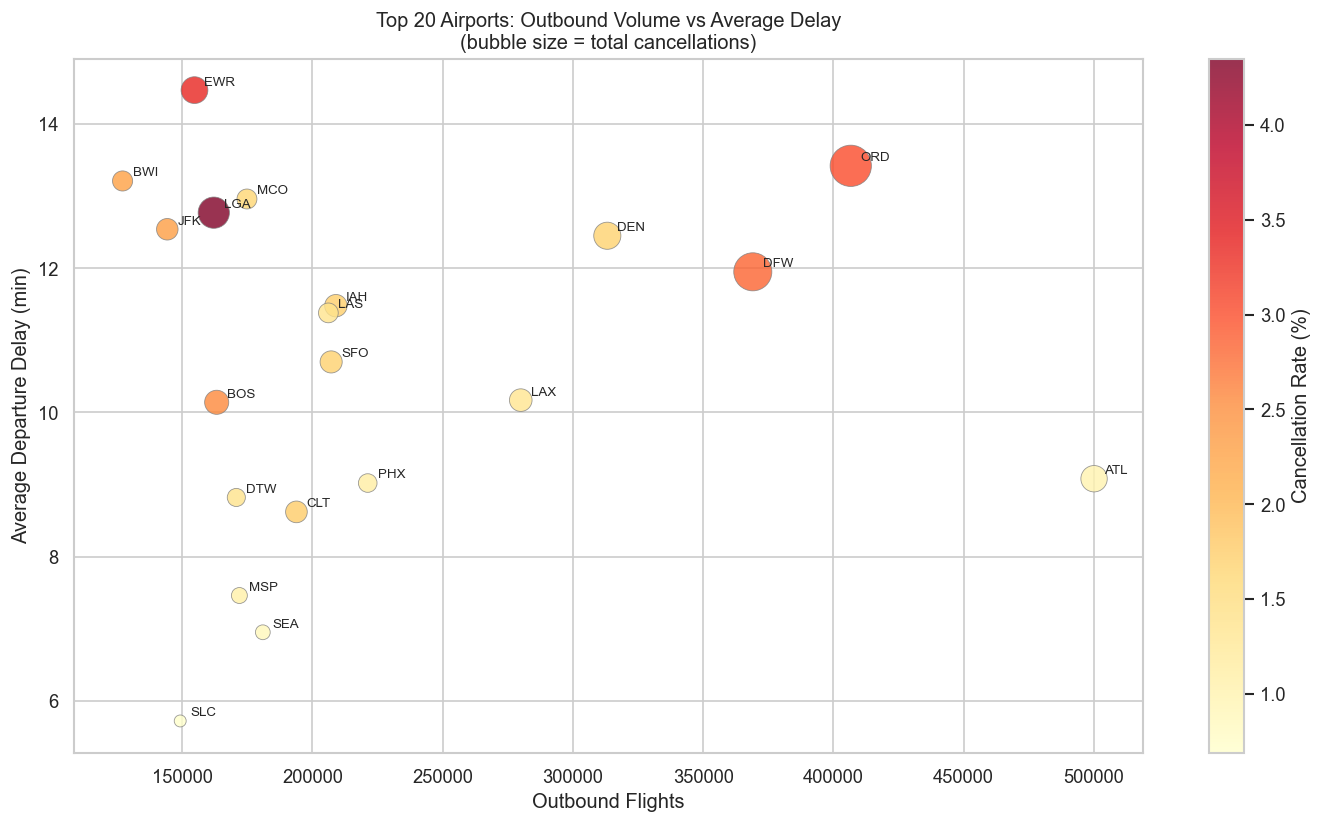
\includegraphics[width=0.9\textwidth]{analysis_6_airports.png}
    \caption{Top 20 airports: outbound volume vs average departure delay. Bubble size = total cancellations; colour = cancellation rate (\%).}
    \label{fig:analysis6}
\end{figure}

\textbf{Full result set:}

\begin{center}
\small
\begin{tabular}{llrrrr}
\toprule
\textbf{IATA} & \textbf{City} & \textbf{Flights} & \textbf{Avg delay} & \textbf{Cancellations} & \textbf{Cancel \%} \\
\midrule
ATL & Atlanta           & 500\,076 &  9.08 &  5\,015 & 1.00 \\
ORD & Chicago           & 406\,670 & 13.42 & 12\,265 & 3.02 \\
DFW & Dallas-Fort Worth & 369\,057 & 11.95 & 10\,430 & 2.83 \\
DEN & Denver            & 313\,203 & 12.45 &  5\,297 & 1.69 \\
LAX & Los Angeles       & 279\,977 & 10.17 &  3\,683 & 1.32 \\
PHX & Phoenix           & 221\,226 &  9.02 &  2\,494 & 1.13 \\
IAH & Houston           & 209\,010 & 11.48 &  3\,613 & 1.73 \\
SFO & San Francisco     & 207\,184 & 10.70 &  3\,525 & 1.70 \\
LAS & Las Vegas         & 206\,114 & 11.38 &  2\,807 & 1.36 \\
CLT & Charlotte         & 193\,856 &  8.62 &  3\,384 & 1.75 \\
SEA & Seattle           & 180\,949 &  6.95 &  1\,577 & 0.87 \\
MCO & Orlando           & 174\,859 & 12.96 &  2\,859 & 1.64 \\
MSP & Minneapolis       & 171\,955 &  7.46 &  1\,834 & 1.07 \\
DTW & Detroit           & 170\,779 &  8.82 &  2\,360 & 1.38 \\
BOS & Boston            & 163\,234 & 10.14 &  4\,180 & 2.56 \\
LGA & New York (LGA)    & 162\,128 & 12.77 &  7\,051 & 4.35 \\
EWR & Newark            & 154\,718 & 14.47 &  5\,161 & 3.34 \\
SLC & Salt Lake City    & 149\,237 &  5.72 &  1\,027 & 0.69 \\
JFK & New York (JFK)    & 144\,277 & 12.54 &  3\,339 & 2.31 \\
BWI & Baltimore         & 127\,109 & 13.21 &  2\,912 & 2.29 \\
\bottomrule
\end{tabular}
\end{center}

\textbf{Key observations:}

\begin{itemize}
    \item \textbf{Atlanta (ATL)} is by far the busiest airport (500\,076
          outbound flights) yet has a below-average delay (9.08~min) and the
          lowest cancellation rate among the top-5 (1.00\%), demonstrating
          that high traffic volume does not necessarily imply poor
          performance.
    \item \textbf{LaGuardia (LGA)} and \textbf{Newark (EWR)} stand out with
          the highest cancellation rates (4.35\% and 3.34\% respectively) and
          among the highest average delays (12.77 and 14.47~min), consistent
          with their known congestion problems in the New York metro airspace.
    \item \textbf{Salt Lake City (SLC)} and \textbf{Seattle (SEA)} are the
          best-performing large airports: SLC averages only 5.72~min departure
          delay with a 0.69\% cancellation rate; SEA averages 6.95~min with
          0.87\%.
    \item \textbf{Chicago O'Hare (ORD)} and \textbf{Dallas-Fort Worth (DFW)}
          combine very high traffic ($>$360\,000 flights each) with elevated
          cancellation rates ($>$2.8\%), confirming their reputation as
          weather- and congestion-prone hubs.
\end{itemize}

\end{document}
